\documentclass[11pt]{article}
\usepackage{amssymb}
\usepackage{algorithm}  
\usepackage{algpseudocode}  
\usepackage{amsmath}  
\usepackage{graphicx}
\renewcommand{\algorithmicrequire}{\textbf{Input:}}  % Use Input in the format of Algorithm  
\renewcommand{\algorithmicensure}{\textbf{Output:}}
\parindent=22pt
\parskip=3pt
\oddsidemargin 18pt \evensidemargin 0pt
\leftmargin 1.5in
\marginparwidth 1in \marginparsep 0pt \headsep 0pt \topskip 20pt
\textheight 225mm \textwidth 148mm
\renewcommand{\baselinestretch}{1.15}
\begin{document}
\title{{\bf The Third Assignment}}
\author{3190102721 Xu Shengze}
\date{}
\maketitle

\begin{tabular*}{13cm}{r}
\hline
\end{tabular*}

\vskip 0.3 in

{\bf Problem 1.} 

a) Calculate the probability to measure the first qubit is state 1 when we have the following 2-qubit system:
$$
\begin{pmatrix}
\frac{1}{2}\\
\frac{-i}{2}\\
\frac{i}{2}\\
\frac{-1}{2}
\end{pmatrix}
$$

b) Calculate the probability to measure the second qubit is state 0 when we have the 
following 2-qubit system:
$$
\begin{pmatrix}
	\frac{1}{3}\\
	\frac{i\sqrt{2}}{3}\\
	\frac{2-i}{3}\\
	\frac{-1}{3}
\end{pmatrix}
$$

c) Calculate the probability to measure the state 11 when we have the following 2-qubit 
system:
$$
\begin{pmatrix}
	0\\
	\frac{1}{3}\\
	\frac{-i}{3}\\
	\frac{2-i\sqrt{3}}{3}
\end{pmatrix}
$$

\vskip 0.3 in

{\bf Answer 1.} By definition, for a 2-qubit system $x=\begin{pmatrix}x_1\\x_2\\x_3\\x_4\end{pmatrix}$, it means the corresponding state $|x\rangle=x_0|00\rangle+x_1|01\rangle+x_2|10\rangle+x_3|11\rangle$, and we have $|x_0|^2+|x_1|^2+|x_2|^2+|x_3|^2=1$.

So the probability to measure the state $00$ is $|x_0|^2$, $01$ is $|x_1|^2$, $10$ is $|x_2|^2$, $11$ is $|x_3|^2$. According to this conclusion, we will solve the three problems in the question.

a) $|x\rangle=\frac{1}{2}|00\rangle+\frac{-i}{2}|01\rangle+\frac{i}{2}|10\rangle+\frac{-1}{2}|11\rangle$. The probability is calculated as follows. 
$$
|\frac{i}{2}|^2+|\frac{-1}{2}|^2=\frac{1}{2}
$$

b) $|x\rangle=\frac{1}{3}|00\rangle+\frac{i\sqrt{2}}{3}|01\rangle+\frac{2-i}{3}|10\rangle+\frac{-1}{3}|11\rangle$. The probability is calculated as follows. 
$$
|\frac{1}{3}|^2+|\frac{2-i}{3}|^2=\frac{2}{3}
$$

c) $|x\rangle=\frac{1}{3}|01\rangle+\frac{-i}{3}|10\rangle+\frac{2-i\sqrt{3}}{3}|11\rangle$. The probability is calculated as follows.
$$
|\frac{2-i\sqrt{3}}{3}|^2=\frac{7}{9}
$$

\vskip 0.3 in

{\bf Problem 2.} 

a) Implement the following classical circuit reversibly:

\begin{figure}[h]
	\centering{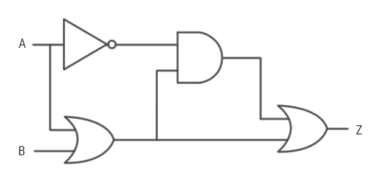
\includegraphics[width=0.4\textwidth]{circuit.png}}
\end{figure}

This circuit can be expressed as ((NOT A) AND (A OR B)) OR (A OR B)

b) Implement this circuit as a quantum circuit by using additional qubits, Toffoli gates and NOT gates.

Remark: in task b) you can consider transforming OR operator into combination of AND 
and NOT operators by using de-Morgan laws.

\vskip 0.3 in

{\bf Answer 2.} 

a) The circuit is as shown below.
\begin{figure}[h]
	\centering{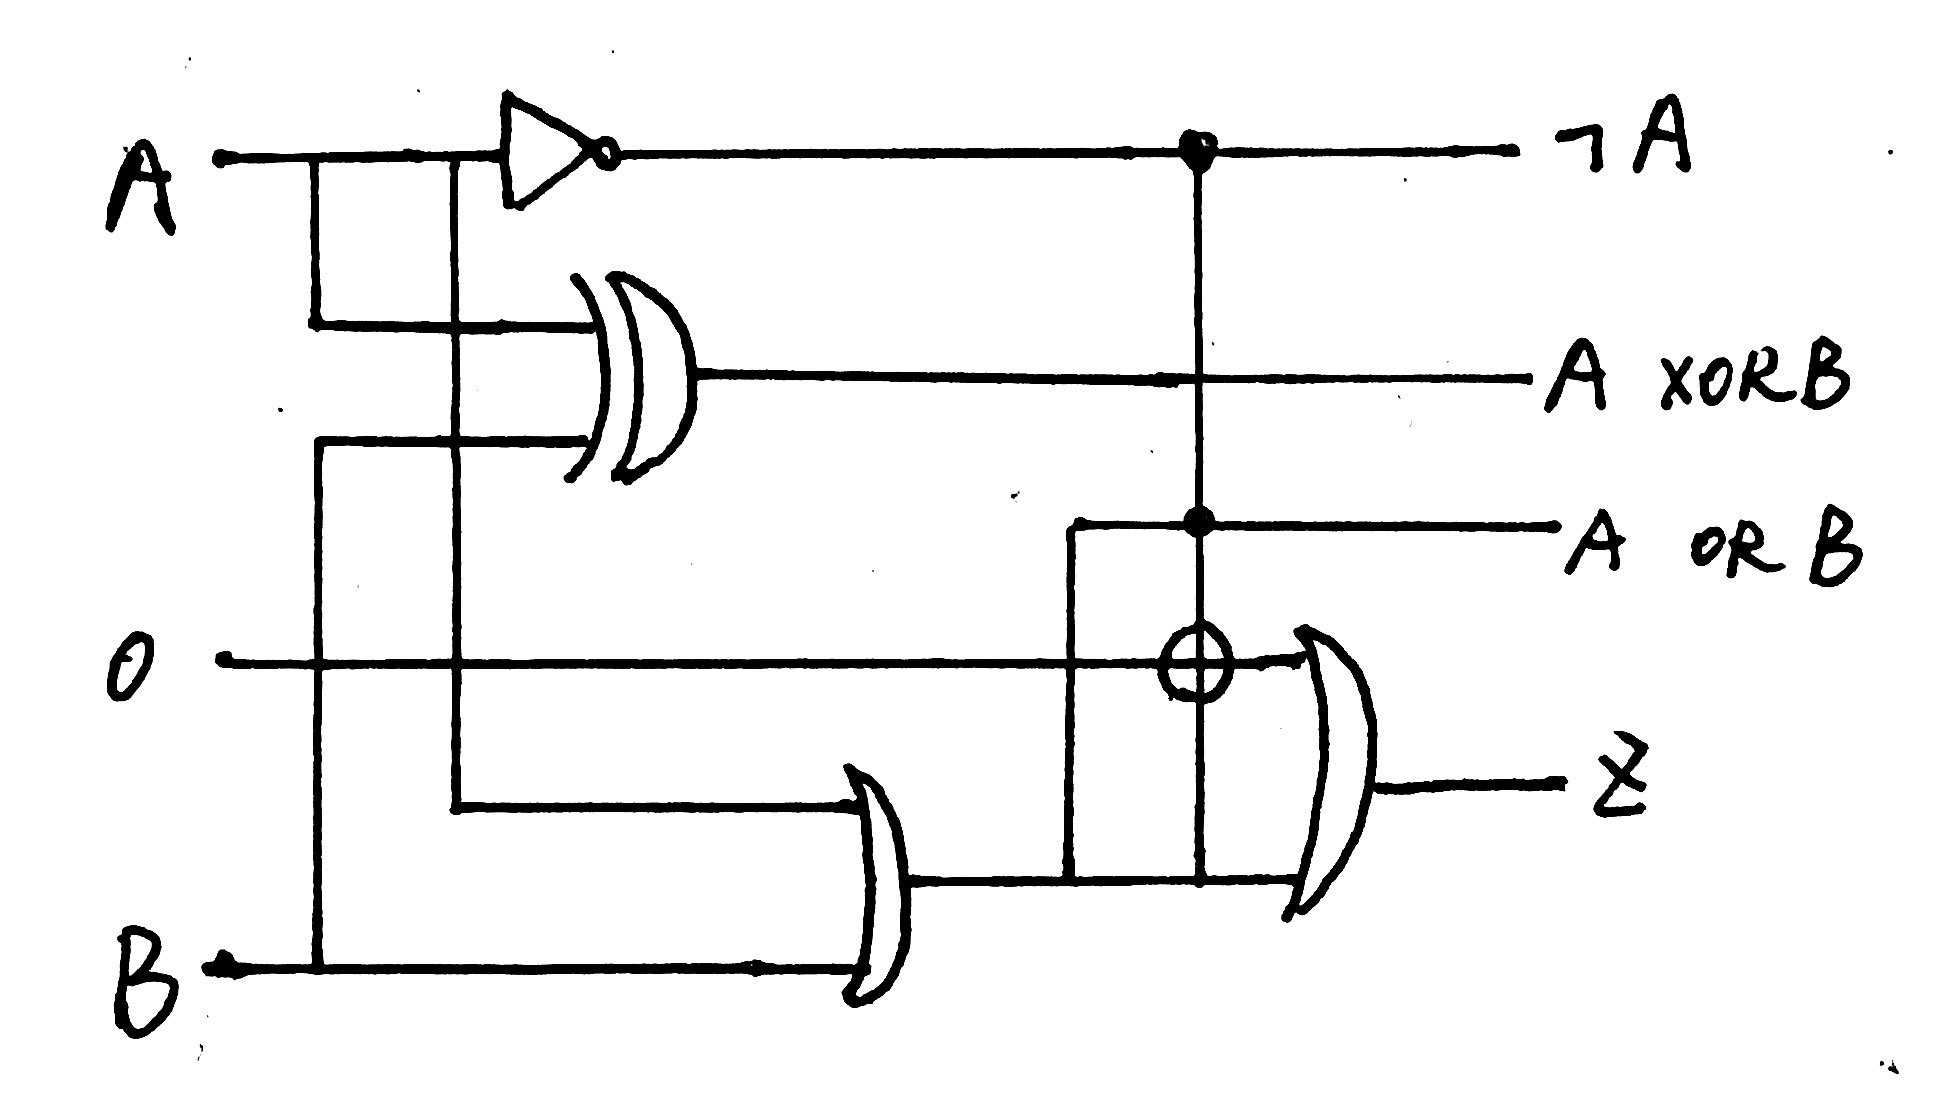
\includegraphics[width=0.5\textwidth]{2a.jpg}}
\end{figure}
\newpage
b) As shown below.
\begin{figure}[!h]
	\centering{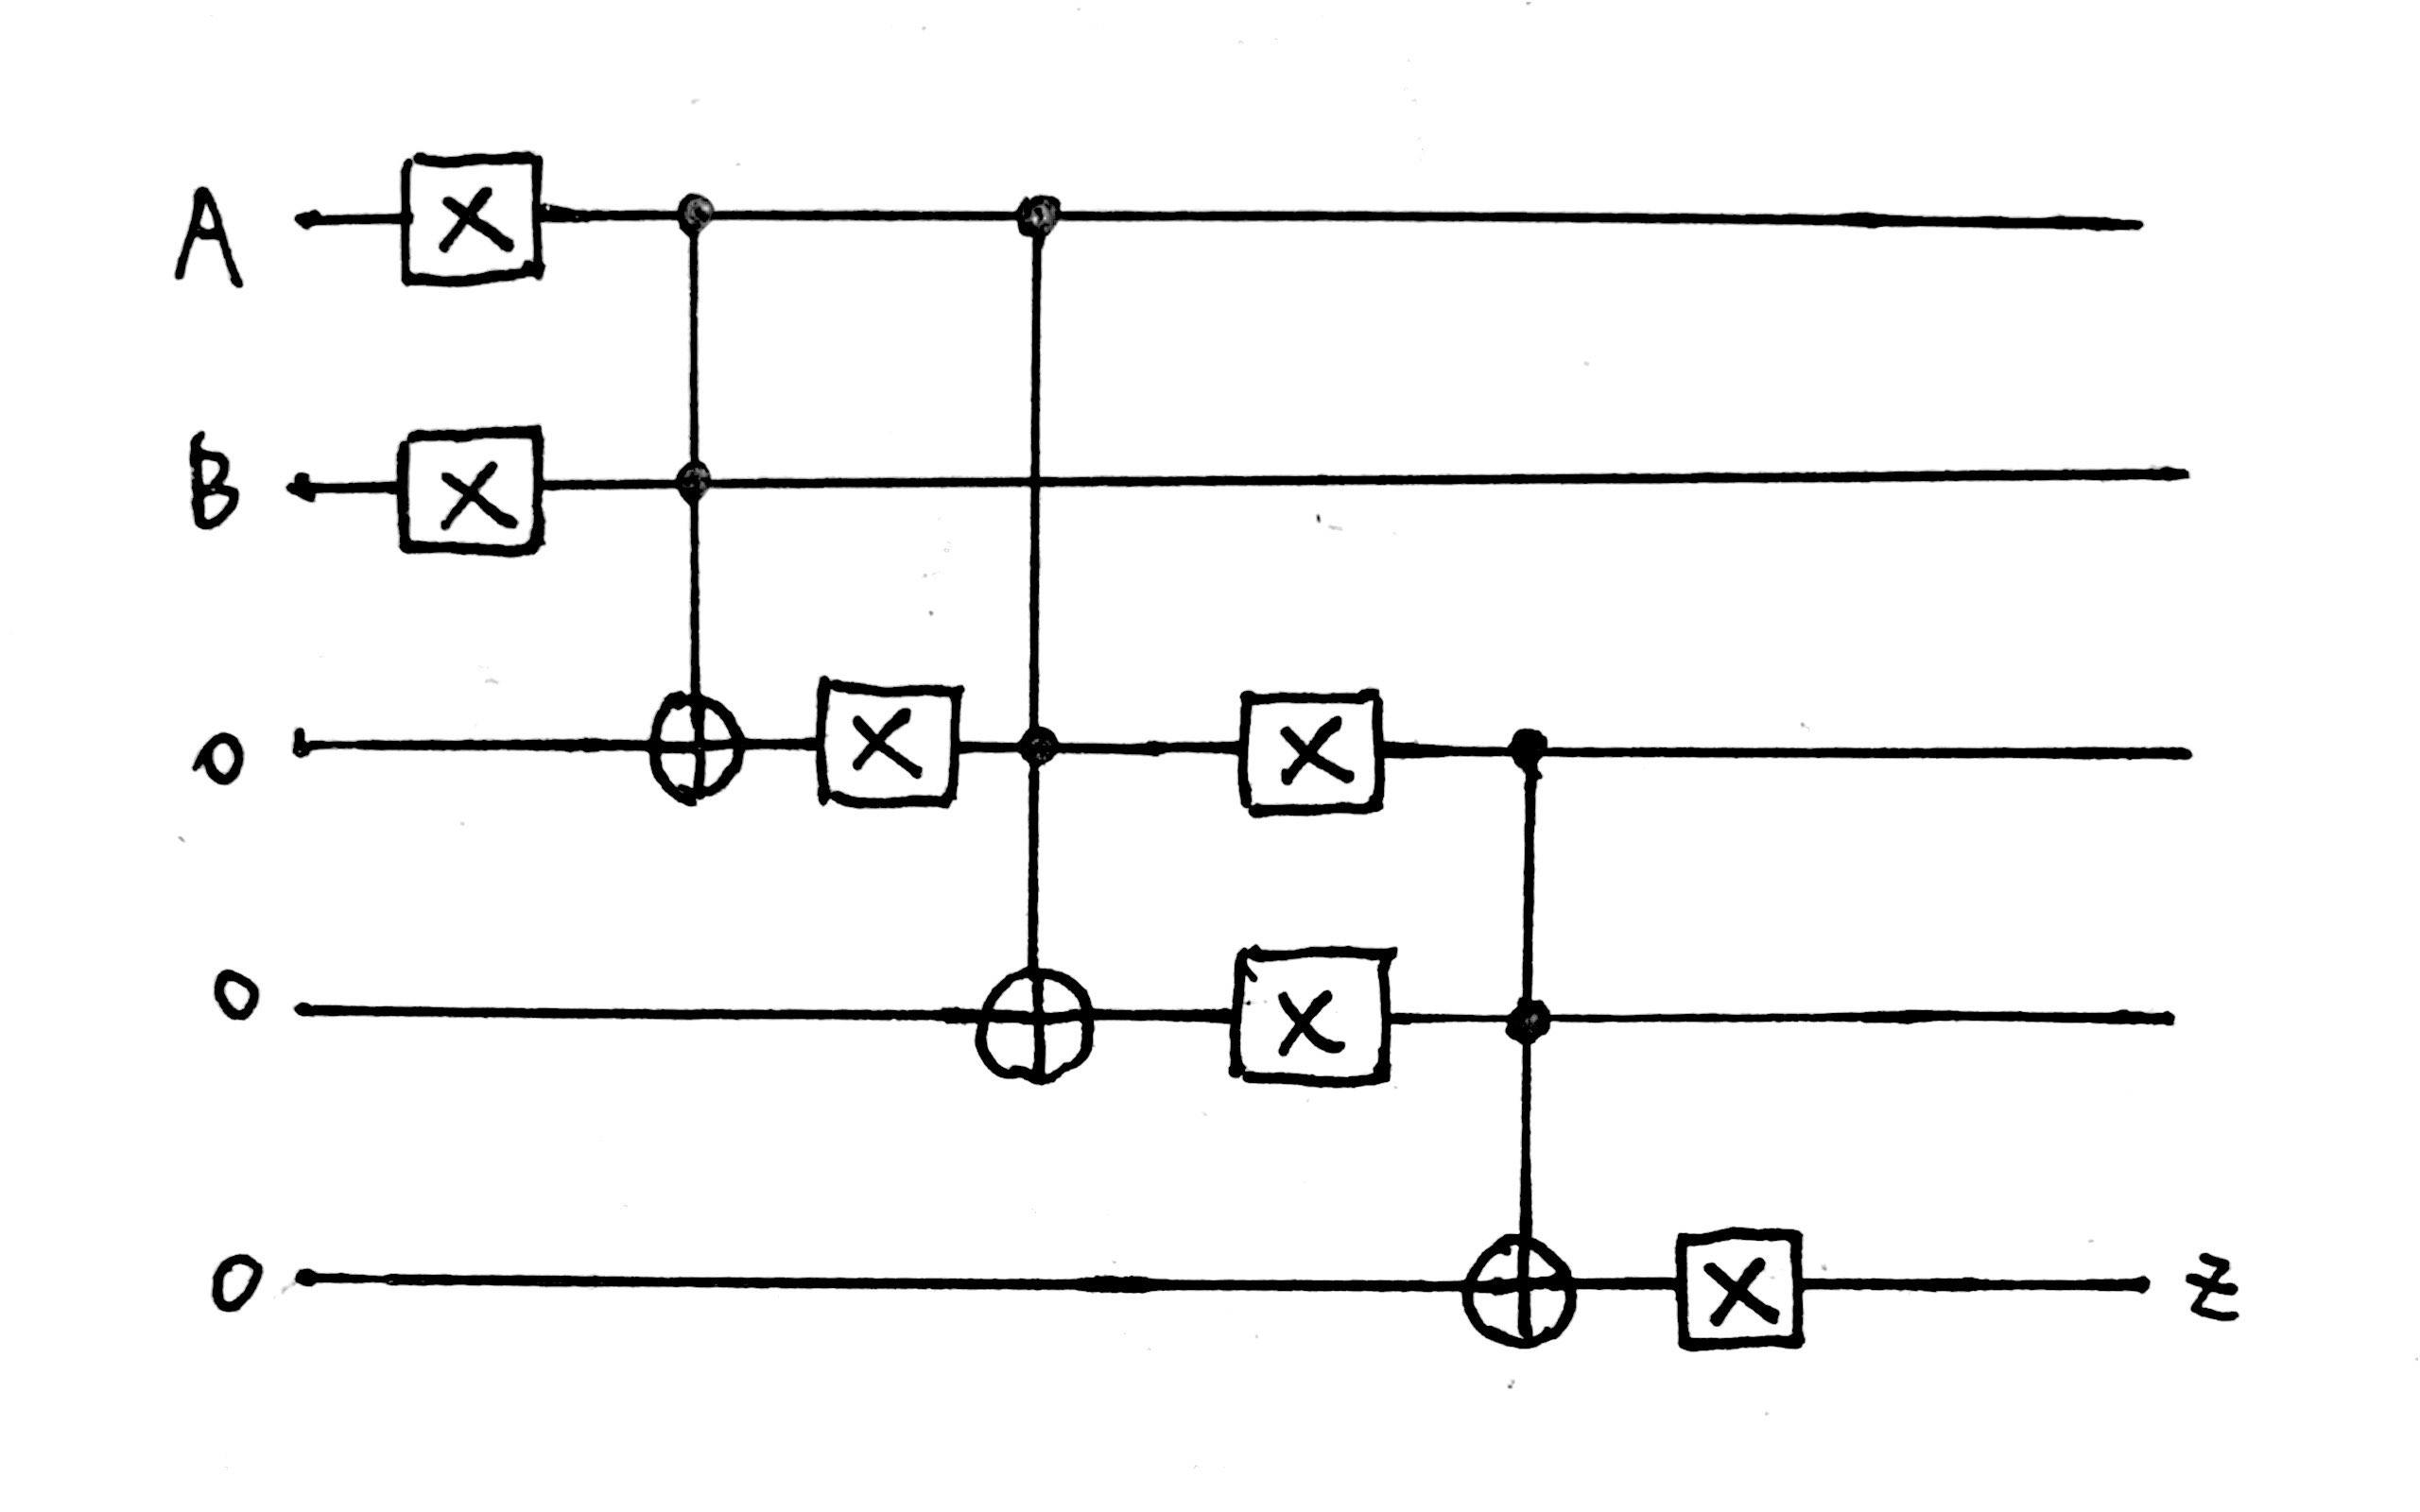
\includegraphics[width=0.5\textwidth]{2b.jpg}}
\end{figure} 

\vskip 0.3 in

{\bf Problem 3.} Implement the quantum circuit that takes values of 8 qubits as input and puts the result of their multiplication in output qubit (which means output is equal to 1 only if all 8 qubits are in state 1; otherwise output is equal to 0). For this task use only Toffoli gates. For this implementation you will need ancilla qubits. Please try to make a circuit that has 15 qubits (8 for input, 6 ancillas and 1 for output).

\vskip 0.3 in

{\bf Answer 3.} The circuit is shown as follows.
\begin{figure}[h]
	\centering{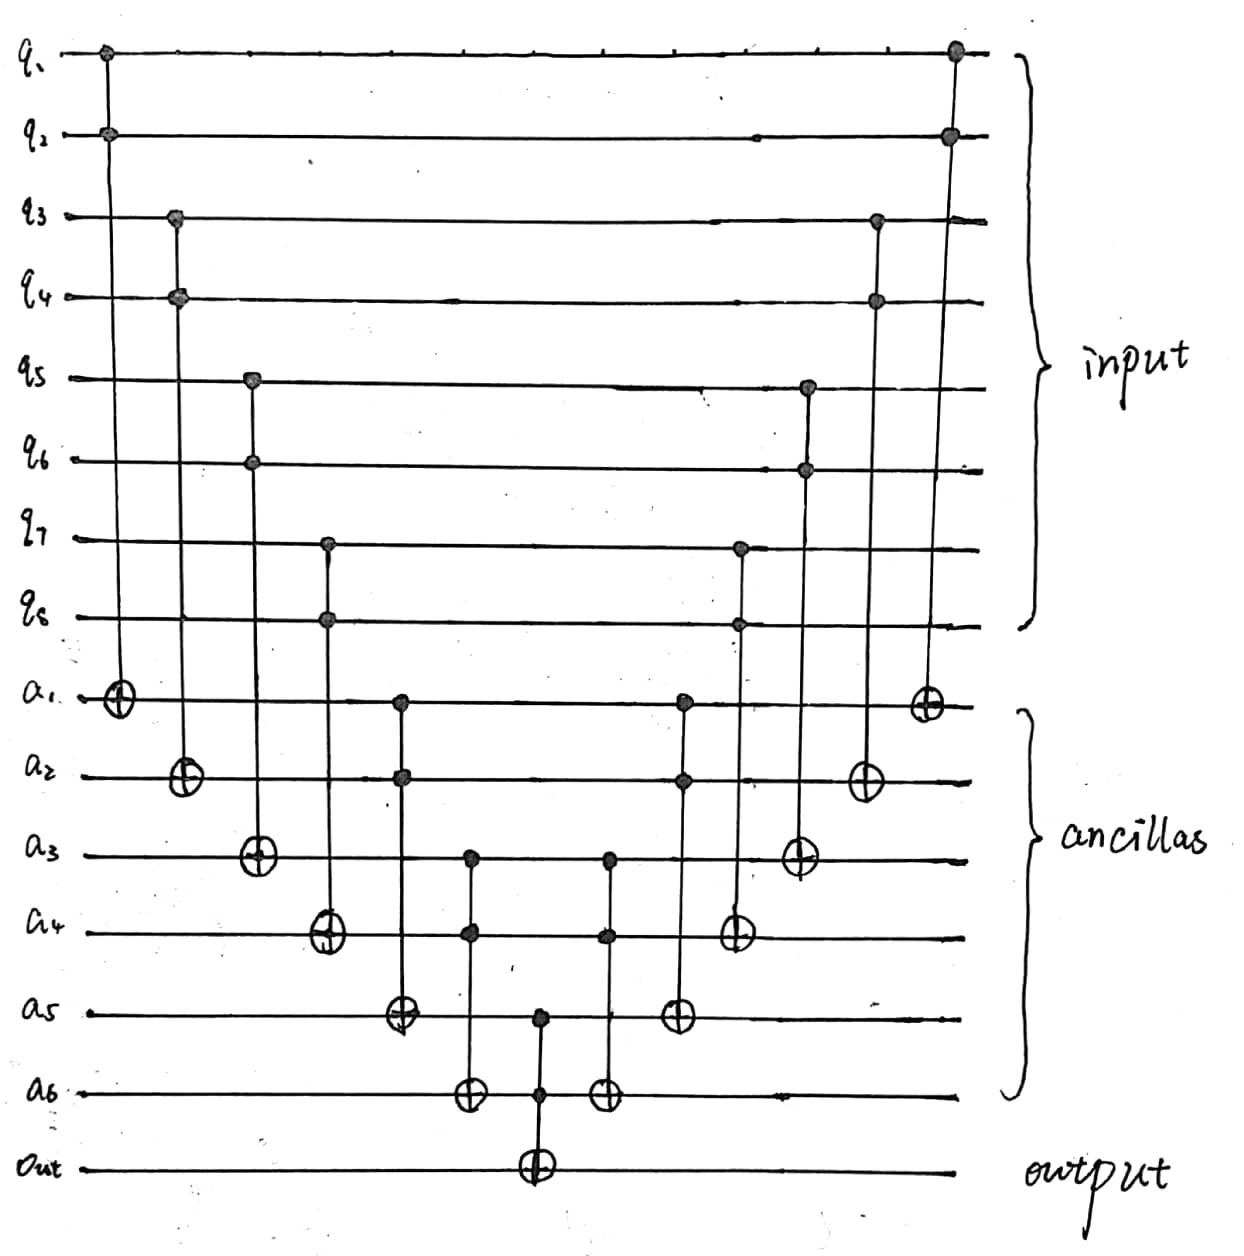
\includegraphics[width=0.7\textwidth]{circuit_3.jpg}}
\end{figure}

\newpage
{\bf Problem 4.} Analyze behavior of Grover’s Search when we have 4 elements and 2 of them are marked. What will be the outcome if we do the measurement after

a) 1 iteration of Grover’s Search for such setting?

b) 2 iterations of Grover’s Search for such setting?

c) 3 iterations of Grover’s Search for such setting?

d) 4 iterations of Grover’s Search for such setting?

Bonus points if you explain behavior of Grover’s Search for cases where exactly half of 
elements in search space is marked.

\vskip 0.3 in

{\bf Answer 4.} The following answers refer to a Chinese textbook on quantum algorithms.

Without loss of generality, we suppose that there are $N$ elements in total and $M$ of them are marked. Then we can represent the state as $|\xi\rangle=\frac{1}{\sqrt{N}}\sum_{x=0}^{N-1}|x\rangle$, where each $x$ represents one element.

Let $S$=\{$x$|the state $|x\rangle$ is marked\}, then $|S|=M$. We define the normalized state as follow,
$$
|\alpha\rangle\equiv\frac{1}{\sqrt{N-M}}\sum_{x\notin S}|x\rangle
$$
$$
|\beta\rangle\equiv\frac{1}{\sqrt{M}}\sum_{x\in S}|x\rangle
$$
simple algebraic operations show that the initial state can be re-expressed as follow,
$$
|\xi\rangle=\sqrt{\frac{N-M}{N}}|\alpha\rangle+\sqrt{\frac{M}{N}}|\beta\rangle
$$

Let $\cos\frac{\theta}{2}=\sqrt{\frac{N-M}{N}}$, then the initial state is $|\xi\rangle=\cos\frac{\theta}{2}|\alpha\rangle+\sin\frac{\theta}{2}|\beta\rangle$, record the initial state as $|\psi_0\rangle$.

a) Let's explain the process of one iteration of Grover's search. 

First, perform operation $O$ on the initial state, where $O(a|\alpha\rangle+b|\beta\rangle)=a|\alpha\rangle-b|\beta\rangle$, then the state will be changed to $|\xi\rangle=\sqrt{\frac{N-M}{N}}|\alpha\rangle-\sqrt{\frac{M}{N}}|\beta\rangle=\cos\frac{\theta}{2}|\alpha\rangle-\sin\frac{\theta}{2}|\beta\rangle$. 

Similarly, the operation $I-2|\xi\rangle\langle\xi|$ also performs a reflection on the plane $|\xi\rangle$ defined by $|\alpha\rangle$ and $|\beta\rangle$, denote this operation as $P$. We apply the above operation to the current state.  This process is equivalent to a symmetrical transformation. After this step, the state becomes $\cos\frac{3\theta}{2}|\alpha\rangle+\sin\frac{3\theta}{2}|\beta\rangle$, which is just the state after one iteration of Grover’s search. We find that the product of the two reflections constitutes a rotation.

Therefore, after one iteration of Grover’s search, the state becomes $|\psi_1\rangle=\cos\frac{3\theta}{2}|\alpha\rangle+\sin\frac{3\theta}{2}|\beta\rangle$. According to $N=4$, $M=2$, we can solve $\theta=\frac{\pi}{2}$, and then we can get the state representation as follows.
$$
|\psi_1\rangle=-\frac{\sqrt{2}}{2}|\alpha\rangle+\frac{\sqrt{2}}{2}|\beta\rangle=-\frac{1}{2}\sum_{x\notin S}|x\rangle+\frac{1}{2}\sum_{x\in S}|x\rangle
$$

So if we do the measurement after 1 iteration of Grover’s Search for such setting, we will have the equal probability of $\frac{1}{4}$ to get each state, each element as well.

For the case where iteration is greater than 1, we discuss and draw general conclusions.  We can prove that after continuous application of $G$ the state becomes as follows.
$$
|\psi_k\rangle=G^k|\psi\rangle=\cos(\frac{2k+1}{2}\theta)|\alpha\rangle+\sin(\frac{2k+1}{2}\theta)|\beta\rangle
$$

We use mathematical induction to prove this conclusion.

(i) When $k=1$, according to the above proof, the conclusion is established.

(ii) Suppose the conclusion holds for $k-1$, then we have $|\psi_{k-1}\rangle=\cos(\frac{2k-1}{2}\theta)|\alpha\rangle+\sin(\frac{2k-1}{2}\theta)|\beta\rangle$. According to the above discussion, $G$ can be regarded as the product of $O$ and $P$, then we do the following operation.
$$
\begin{aligned}
|\psi_k\rangle=G|\psi_{k-1}\rangle&=P(O|\psi_{k-1}\rangle)\\
&=P(\cos(-\frac{2k-1}{2}\theta)|\alpha\rangle+\sin(-\frac{2k-1}{2}\theta)|\beta\rangle)\\
&=\cos(\frac{2k+1}{2}\theta)|\alpha\rangle+\sin(\frac{2k+1}{2}\theta)|\beta\rangle
\end{aligned}
$$

Therefore the conclusion holds for $k$, then the conclusion is correct. Below we apply this conclusion to solve problem b, c, d.

b) After 2 iterations of Grover’s Search for such setting, there are the following results. 
$$
|\psi_2\rangle=-\frac{\sqrt{2}}{2}|\alpha\rangle-\frac{\sqrt{2}}{2}|\beta\rangle=-\frac{1}{2}\sum_{x\notin S}|x\rangle-\frac{1}{2}\sum_{x\in S}|x\rangle
$$ 

c) After 3 iterations of Grover’s Search for such setting, there are the following results. 
$$
|\psi_3\rangle=\frac{\sqrt{2}}{2}|\alpha\rangle-\frac{\sqrt{2}}{2}|\beta\rangle=\frac{1}{2}\sum_{x\notin S}|x\rangle-\frac{1}{2}\sum_{x\in S}|x\rangle
$$

d) After 4 iterations of Grover’s Search for such setting, there are the following results. 
$$
|\psi_4\rangle=\frac{\sqrt{2}}{2}|\alpha\rangle+\frac{\sqrt{2}}{2}|\beta\rangle=\frac{1}{2}\sum_{x\notin S}|x\rangle+\frac{1}{2}\sum_{x\in S}|x\rangle
$$


For the three questions b, c and d, we have the same conclusion. If we do the measurement after either 2 or 3 or 4 iterations of Grover’s Search for such setting, we will have the equal probability of $\frac{1}{4}$ to get each state, each element as well.

\textbf{Bonus: }If half of elements in search space is marked, then $M=\frac{N}{2}$, so $\theta=\frac{\pi}{2}$, then based on the above discussion, we have the following conclusions.
$$
|\psi_k\rangle=\pm\frac{\sqrt{2}}{2}|\alpha\rangle\pm\frac{\sqrt{2}}{2}|\beta\rangle=\pm\frac{1}{\sqrt{N}}\sum_{x\notin S}|x\rangle\pm\frac{1}{\sqrt{N}}\sum_{x\in S}|x\rangle
$$

So when doing the measurement, we will have the equal probability of $\frac{1}{N}$ to get each state, each element as well. It is the behavior of Grover’s Search for this case.
\end{document}
